\documentclass[a4paper,12pt]{report}

%% Color
\usepackage{color}

%% Diagrams
\usepackage{graphicx,epsfig}

%% To control the table caption positioning
\usepackage{caption} 
\captionsetup[table]{skip=5pt}

%% 'H' for exact placement of floats
\usepackage{float}

%% For a lot of maths support, including align
\usepackage{amsmath}

%% For euros
\usepackage{eurosym}

%% Bibliography
\usepackage[round]{natbib}

%% Make bib references, URLs, etc into hyperlinks
\usepackage[hidelinks]{hyperref}
\hypersetup{colorlinks,linkcolor={blue},citecolor={blue},urlcolor={blue}}

%% Personalisation
\setlength{\parskip}{1em}

%% Show Great Dedication
\newenvironment{dedication}
    {\vspace{6ex}\begin{quotation}\begin{center}\begin{em}}
    {\par\end{em}\end{center}\end{quotation}}

\begin{document}

\author{\textbf{Devrim Gunyel}\\[1ex]
  Department of Computer Science\\
  Maynooth University\\
  Maynooth\\
  Co. Kildare\\
  IRELAND}
\date{\today}
\title{Identifying Signs of Diabetic Retinopathy Using Deep Learning}
\maketitle

%% Acknowledgement, Dedication and Declaration will be added here. Currently I can not add titles?????? 
\begin{center}\begin{em}}
To Yazidi women...
{\par\end{em}\end{center}}
\section*{Declaration}
I  declare  that  the  dissertation thesis and  code  for  ‘Identifying Signs of Diabetic Retinopathy’ submitted for assessment is my own work except where credit is explicitly given to others by citation or acknowledgement. This work was accomplished during  the  current  academic  year  except  where  otherwise stated. 

In  submitting  this  project  report  to  the  National University of Maynooth,  I hereby give permission for it to be made available for use in accordance with the regulations of the University Library. I also give permission for the title and abstract to be published  and  for  copies of  the  report  to be  made  and  supplied  at cost to  any bona  fide  library  or  research  worker,  and  to  be  made  available  on  the  World Wide Web. 
In addition, I retain the copyright to this work. 
\section*{Acknowledgements}
And I would like to acknowledge....

\begin{abstract}

Diabetic Retinopathy is a visual impairment disease as a result of diabetes mellitus. Visual impairment caused by diabetic retinopathy(DR) can be cured if detected in earlier stage of DR in patients. In this work, we try to automatically detect signs of DR by using deep neural networks. For this purpose, we train deep neural network by using one of the widely used publicly available datasets and test with other public datasets. Experimental results show that deep learning techniques can be promising in the task of automatic detection of DR.    

WILL BE EXTENDED

\end{abstract}


\tableofcontents

\newpage

%*******************************************************************************
%*********************************** First Chapter *****************************
%*******************************************************************************

\chapter{Getting started}  %Title of the First Chapter

\ifpdf
    \graphicspath{{Chapter1/Figs/Raster/}{Chapter1/Figs/PDF/}{Chapter1/Figs/}}
\else
    \graphicspath{{Chapter1/Figs/Vector/}{Chapter1/Figs/}}
\fi


%********************************** %First Section  **************************************
\section{What is loren ipsum? Title with math \texorpdfstring{$\sigma$}{[sigma]}} %Section - 1.1 

Lorem Ipsum is simply dummy text of the printing and typesetting industry (see 
Section~\ref{section1.3}). Lorem Ipsum~\citep{Aup91} has been the industry's 
standard dummy text ever since the 1500s, when an unknown printer took a galley 
of type and scrambled it to make a type specimen book. It has survived not only 
five centuries, but also the leap into electronic typesetting, remaining 
essentially unchanged. It was popularised in the 1960s with the release of 
Letraset sheets containing Lorem Ipsum passages, and more recently with desktop 
publishing software like Aldus PageMaker including versions of Lorem 
Ipsum~\citep{AAB95,Con90,LM65}.

The most famous equation in the world: $E^2 = (m_0c^2)^2 + (pc)^2$, which is 
known as the \textbf{energy-mass-momentum} relation as an in-line equation.

A {\em \LaTeX{} class file}\index{\LaTeX{} class file@LaTeX class file} is a file, which holds style information for a particular \LaTeX{}.


\begin{align}
CIF: \hspace*{5mm}F_0^j(a) = \frac{1}{2\pi \iota} \oint_{\gamma} \frac{F_0^j(z)}{z - a} dz
\end{align}

\nomenclature[z-cif]{$CIF$}{Cauchy's Integral Formula}                                % first letter Z is for Acronyms 
\nomenclature[a-F]{$F$}{complex function}                                                   % first letter A is for Roman symbols
\nomenclature[g-p]{$\pi$}{ $\simeq 3.14\ldots$}                                             % first letter G is for Greek Symbols
\nomenclature[g-i]{$\iota$}{unit imaginary number $\sqrt{-1}$}                      % first letter G is for Greek Symbols
\nomenclature[g-g]{$\gamma$}{a simply closed curve on a complex plane}  % first letter G is for Greek Symbols
\nomenclature[x-i]{$\oint_\gamma$}{integration around a curve $\gamma$} % first letter X is for Other Symbols
\nomenclature[r-j]{$j$}{superscript index}                                                       % first letter R is for superscripts
\nomenclature[s-0]{$0$}{subscript index}                                                        % first letter S is for subscripts


%********************************** %Second Section  *************************************
\section{Why do we use loren ipsum?} %Section - 1.2


It is a long established fact that a reader will be distracted by the readable content of a page when looking at its layout. The point of using Lorem Ipsum is that it has a more-or-less normal distribution of letters, as opposed to using `Content here, content here', making it look like readable English. Many desktop publishing packages and web page editors now use Lorem Ipsum as their default model text, and a search for `lorem ipsum' will uncover many web sites still in their infancy. Various versions have evolved over the years, sometimes by accident, sometimes on purpose (injected humour and the like).

%********************************** % Third Section  *************************************
\section{Where does it come from?}  %Section - 1.3 
\label{section1.3}

Contrary to popular belief, Lorem Ipsum is not simply random text. It has roots in a piece of classical Latin literature from 45 BC, making it over 2000 years old. Richard McClintock, a Latin professor at Hampden-Sydney College in Virginia, looked up one of the more obscure Latin words, consectetur, from a Lorem Ipsum passage, and going through the cites of the word in classical literature, discovered the undoubtable source. Lorem Ipsum comes from sections 1.10.32 and 1.10.33 of "de Finibus Bonorum et Malorum" (The Extremes of Good and Evil) by Cicero, written in 45 BC. This book is a treatise on the theory of ethics, very popular during the Renaissance. The first line of Lorem Ipsum, "Lorem ipsum dolor sit amet..", comes from a line in section 1.10.32.

The standard chunk of Lorem Ipsum used since the 1500s is reproduced below for those interested. Sections 1.10.32 and 1.10.33 from ``de Finibus Bonorum et Malorum" by Cicero are also reproduced in their exact original form, accompanied by English versions from the 1914 translation by H. Rackham

``Lorem ipsum dolor sit amet, consectetur adipisicing elit, sed do eiusmod tempor incididunt ut labore et dolore magna aliqua. Ut enim ad minim veniam, quis nostrud exercitation ullamco laboris nisi ut aliquip ex ea commodo consequat. Duis aute irure dolor in reprehenderit in voluptate velit esse cillum dolore eu fugiat nulla pariatur. Excepteur sint occaecat cupidatat non proident, sunt in culpa qui officia deserunt mollit anim id est laborum."

Section 1.10.32 of ``de Finibus Bonorum et Malorum", written by Cicero in 45 BC: ``Sed ut perspiciatis unde omnis iste natus error sit voluptatem accusantium doloremque laudantium, totam rem aperiam, eaque ipsa quae ab illo inventore veritatis et quasi architecto beatae vitae dicta sunt explicabo. Nemo enim ipsam voluptatem quia voluptas sit aspernatur aut odit aut fugit, sed quia consequuntur magni dolores eos qui ratione voluptatem sequi nesciunt. Neque porro quisquam est, qui dolorem ipsum quia dolor sit amet, consectetur, adipisci velit, sed quia non numquam eius modi tempora incidunt ut labore et dolore magnam aliquam quaerat voluptatem. Ut enim ad minima veniam, quis nostrum exercitationem ullam corporis suscipit laboriosam, nisi ut aliquid ex ea commodi consequatur? Quis autem vel eum iure reprehenderit qui in ea voluptate velit esse quam nihil molestiae consequatur, vel illum qui dolorem eum fugiat quo voluptas nulla pariatur?"

1914 translation by H. Rackham: ``But I must explain to you how all this mistaken idea of denouncing pleasure and praising pain was born and I will give you a complete account of the system, and expound the actual teachings of the great explorer of the truth, the master-builder of human happiness. No one rejects, dislikes, or avoids pleasure itself, because it is pleasure, but because those who do not know how to pursue pleasure rationally encounter consequences that are extremely painful. Nor again is there anyone who loves or pursues or desires to obtain pain of itself, because it is pain, but because occasionally circumstances occur in which toil and pain can procure him some great pleasure. To take a trivial example, which of us ever undertakes laborious physical exercise, except to obtain some advantage from it? But who has any right to find fault with a man who chooses to enjoy a pleasure that has no annoying consequences, or one who avoids a pain that produces no resultant pleasure?"

Section 1.10.33 of ``de Finibus Bonorum et Malorum", written by Cicero in 45 BC: ``At vero eos et accusamus et iusto odio dignissimos ducimus qui blanditiis praesentium voluptatum deleniti atque corrupti quos dolores et quas molestias excepturi sint occaecati cupiditate non provident, similique sunt in culpa qui officia deserunt mollitia animi, id est laborum et dolorum fuga. Et harum quidem rerum facilis est et expedita distinctio. Nam libero tempore, cum soluta nobis est eligendi optio cumque nihil impedit quo minus id quod maxime placeat facere possimus, omnis voluptas assumenda est, omnis dolor repellendus. Temporibus autem quibusdam et aut officiis debitis aut rerum necessitatibus saepe eveniet ut et voluptates repudiandae sint et molestiae non recusandae. Itaque earum rerum hic tenetur a sapiente delectus, ut aut reiciendis voluptatibus maiores alias consequatur aut perferendis doloribus asperiores repellat."

1914 translation by H. Rackham: ``On the other hand, we denounce with righteous indignation and dislike men who are so beguiled and demoralized by the charms of pleasure of the moment, so blinded by desire, that they cannot foresee the pain and trouble that are bound to ensue; and equal blame belongs to those who fail in their duty through weakness of will, which is the same as saying through shrinking from toil and pain. These cases are perfectly simple and easy to distinguish. In a free hour, when our power of choice is untrammelled and when nothing prevents our being able to do what we like best, every pleasure is to be welcomed and every pain avoided. But in certain circumstances and owing to the claims of duty or the obligations of business it will frequently occur that pleasures have to be repudiated and annoyances accepted. The wise man therefore always holds in these matters to this principle of selection: he rejects pleasures to secure other greater pleasures, or else he endures pains to avoid worse pains."

\chapter{Related Work} \label{related_work}

Details what others have done that is relevant to your work. \ref{intro}.
\begin{enumerate}
    \item Objectives
    \item Describe the context of the research question in detail, defining terminology, and with references.
    \item Explain how the problem, or related problems, has been solved previously. Critically analyze existing solutions. Discuss how your approach compares to these solutions.
    \item Explain other techniques that you have used to: help understand and analyze the research question; motivate your own work; evaluate your solution.
\end{enumerate}
\section{Objectives}
A single sentence that describes the purpose of this section.
\section{Eye Disease Datasets}
\subsection{Feature Datasets}
- Clinical trial dataset'e bak
- From Messidor fundus image, extracted features 
\subsection{Diabetic Retinopathy Fundus Image Datasets}

\citet{kauppi2013constructing} addressed \citet{thacker2008performance}'s 8 key questions for 6 publicly available fundus image databases. These questions are:

\begin{enumerate}
    \item How is testing currently performed?
    \item Is there a data set for which the correct answers are known?
    \item Are there data sets in common use?
    \item Are there experiments which show algorithms are stable and work as expected?
    \item Are there any strawman algorithms?
    \item What code and data are available?
    \item Is there a quantitative methodology for the design of algorithms?
    \item What should we be measuring to quantify performance? What metrics are used?
\end{enumerate}

In his research, he compared these 6 databases and summarised them depends on amount of these addressed questions \citep{kauppi2013constructing}. Also, in his thesis he established DIARETDB1 database by means of these key questions.

In this section, I give information about some of the publicly available fundus image databases.

\subsubsection{DRIVE (Digital Retinal Images for Vessel Extraction)}
DRIVE data set constructed by \citet{staal2004ridge}.
DRIVE data set includes 40 manually labelled retinal images for training and evaluation of \citet{staal2004ridge}'s method which are randomly selected from 400 diabetic subjects between 25-90 years of age as a part of a screening programme in the Netherlands. Images labelled by 3 human observers who were trained by experienced ophthalmologist. 7 of these manually labelled retinal images has DR indications and 33 of them not. 

DRIVE addresses 7 of \citet{kauppi2013constructing}'s key questions which is one of the best results if you compare with the other 6 databases. It makes publicly available DRIVE very popular in automated diabetic retinopaty detection environment.

General information about DRIVE database:
\begin{itemize}
    \item \textbf{Availability date: } 2004
    \item \textbf{Size: } 40 retinal images
    \item \textbf{DR Size: } 7 retinal images
    \item \textbf{Non-DR Size: } 33 retinal images
    \item \textbf{Camera: } Canon CR5 non-mydriatic 3CCD camera with a 45 degree field of view
    \item \textbf{Resolution: } 768 by 584 pixels
\end{itemize}

\subsubsection{STARE (STructured Analysis of the Retina)}
Stare database contains ~400 publicly available raw images which can be obtained from STARE website \citep{STARE}. They also gives a list of information about diagnosis of these images. They also shared 20 hand labelled images for blood vessel segmentation \citep{hoover2000locating} extracted from these ~400 images. Because I can obtain DR, non-DR information from diagnosis list. There are 13 diagnosis which represented with numbers in the list. The images which has DR diagnosis represented with 7 and 8 which addresses Background Diabetic Retinopathy(BDR/NPDR) and Proliferative Diabetic Retinopathy(PDR). These diagnosis and their diagnosis numbers can be found on appendix. {APPENDIX EKLE!!!!} - diagnosis listesini ve image-diagnosis listesini.

General information about STARE database:

\begin{itemize}
    \item \textbf{Availability date: } 2004
    \item \textbf{Size: } 397 retinal images
    \item \textbf{DR Size: } 10 retinal images
    \item \textbf{Non-DR Size: } 10 retinal images
    \item \textbf{Camera: } TopCon TRV-50 fundus camera with a 35 degree field of view
    \item \textbf{Resolution: } 605 by 700 pixels
\end{itemize}

\subsubsection{CHASE (Child Heart And Health Study in England)}

CHASEDB, retinal vessel reference data-set, includes 28 retinal fundus images of 14 multiethnic children's (aged 10 years) both eyes during September 2007 in North-East London as a part of \citep{fraz2012ensemble}. As we mentioned in Chapter \ref{intro}, detecting neovascularisation is another way of diagnosing DR. CHASEDB mostly used for detection of blood vessels \citep{liskowski2016segmenting} \citep{elbalaoui2016automatic}. There is not any information about DR on these images and I am not checking information related with blood vessels so I did not considered this database in my experiments.

General information about CHASE database:
\begin{itemize}
    \item \textbf{Availability date: } 2012
    \item \textbf{Size: } 28 retinal images
    \item \textbf{Camera: } NM-200-D fundus camera with 30 degree field of view made bu Nidek Co. Ltd., Gamagori, Japan
    \item \textbf{Resolution: } 1280 by 960 pixels
\end{itemize}

\subsubsection{ROC}
General information about ROC database:
\begin{itemize}
    \item \textbf{Availability date: } 2004
    \item \textbf{Size: } 40 retinal images
    \item \textbf{DR Size: } 7 retinal images
    \item \textbf{Non-DR Size: } 33 retinal images
    \item \textbf{Camera: } Canon CR5 non-mydriatic 3CCD camera with a 45 degree field of view
    \item \textbf{Resolution: } 768 by 584 pixels
\end{itemize}

\subsubsection{E-Optha}
\subsubsection{HRFDB}

\subsubsection{CMIF}
General information about CMIF database:
\begin{itemize}
    \item \textbf{Availability date: } 2004
    \item \textbf{Size: } 40 retinal images
    \item \textbf{DR Size: } 7 retinal images
    \item \textbf{Non-DR Size: } 33 retinal images
    \item \textbf{Camera: } Canon CR5 non-mydriatic 3CCD camera with a 45 degree field of view
    \item \textbf{Resolution: } 768 by 584 pixels
\end{itemize}

\subsubsection{REVIEW}
General information about REVIEW database:
\begin{itemize}
    \item \textbf{Availability date: } 2004
    \item \textbf{Size: } 40 retinal images
    \item \textbf{DR Size: } 7 retinal images
    \item \textbf{Non-DR Size: } 33 retinal images
    \item \textbf{Camera: } Canon CR5 non-mydriatic 3CCD camera with a 45 degree field of view
    \item \textbf{Resolution: } 768 by 584 pixels
\end{itemize}

\subsubsection{DIARETDB}
General information about DIARETDB0 database:
\begin{itemize}
    \item \textbf{Availability date: } 2004
    \item \textbf{Size: } 40 retinal images
    \item \textbf{DR Size: } 7 retinal images
    \item \textbf{Non-DR Size: } 33 retinal images
    \item \textbf{Camera: } Canon CR5 non-mydriatic 3CCD camera with a 45 degree field of view
    \item \textbf{Resolution: } 768 by 584 pixels
\end{itemize}

General information about DIARETDB1 database:
\begin{itemize}
    \item \textbf{Availability date: } 2004
    \item \textbf{Size: } 40 retinal images
    \item \textbf{DR Size: } 7 retinal images
    \item \textbf{Non-DR Size: } 33 retinal images
    \item \textbf{Camera: } Canon CR5 non-mydriatic 3CCD camera with a 45 degree field of view
    \item \textbf{Resolution: } 768 by 584 pixels
\end{itemize}

General information about DIARETDB2 database:
\begin{itemize}
    \item \textbf{Availability date: } 2004
    \item \textbf{Size: } 40 retinal images
    \item \textbf{DR Size: } 7 retinal images
    \item \textbf{Non-DR Size: } 33 retinal images
    \item \textbf{Camera: } Canon CR5 non-mydriatic 3CCD camera with a 45 degree field of view
    \item \textbf{Resolution: } 768 by 584 pixels
\end{itemize}

\subsubsection{MESSIDOR}
General information about MESSIDOR database:
\begin{itemize}
    \item \textbf{Availability date: } 2004
    \item \textbf{Size: } 40 retinal images
    \item \textbf{DR Size: } 7 retinal images
    \item \textbf{Non-DR Size: } 33 retinal images
    \item \textbf{Camera: } Canon CR5 non-mydriatic 3CCD camera with a 45 degree field of view
    \item \textbf{Resolution: } 768 by 584 pixels
\end{itemize}

\section{Machine Leearning Approaches for Diabetic Retinopathy}
\subsection{Other Approaches}
\subsection{Neural Network Approaches for Diabetic Retinpathy}

\chapter{Solution}
\begin{enumerate}
    \item often the name of your solution - details what you have done and how you have done it.
    \item objectives - a single sentence that describes the purpose of this section
    \item provide an analysis of the problem , motivating your approach to answering the research question.
    \item Explain your approach by describing exactly what you have done.
    \item Explain how you have achieved your solution. Examples: explain how a process improvement was implemented, how a mathematical technique was derived, or how an algorithm was implemented.
\end{enumerate}

\section{Background}
\subsection{Deep Learning}
Deep Learning is defined as:
``A class of machine learning techniques that exploit many layers of non-linear information processing for supervised or unsupervised feature extraction and transformation, and for pattern analysis and classification''
by \citet[][\emph{Deep Learning Methods and Applications}]{deng2014deep}. In this work we investigate the effects of using Deep Learning techniques for the task of finding the signs of diabetic retinopathy and for this task we use a special type of Artificial Neural Networks called Convolutional Neural Networks that we will explain in detail in the following sections.   

\begin{figure}[t]
\centering
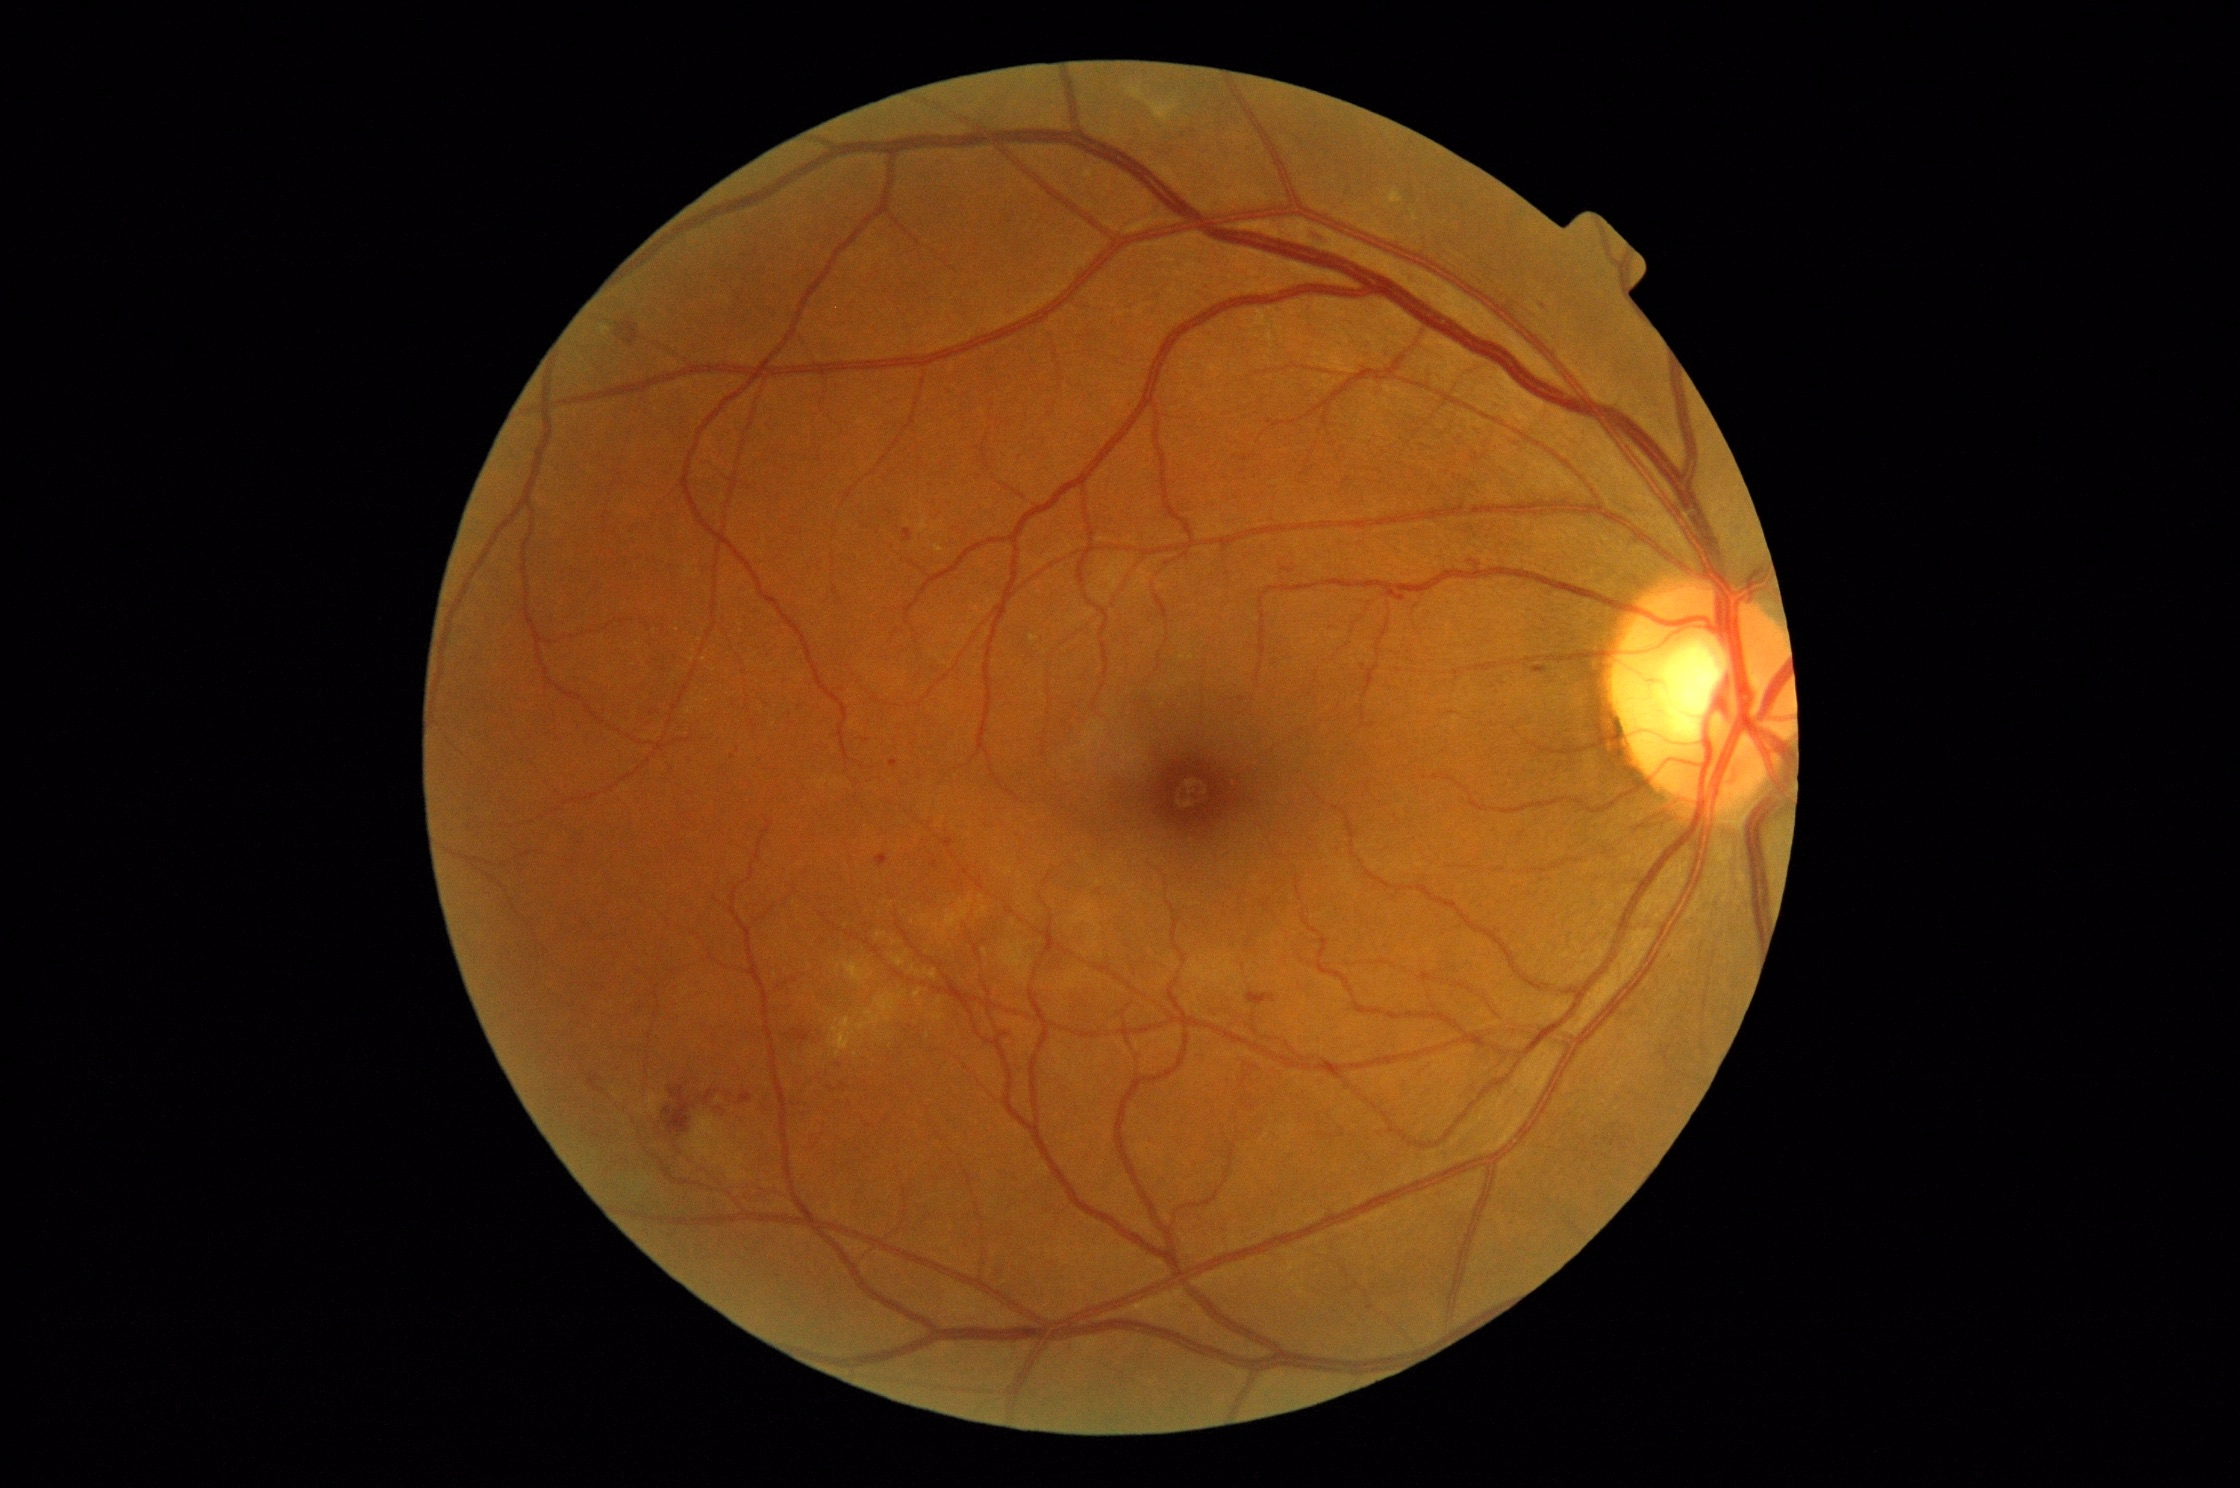
\includegraphics[width=0.8\textwidth]{Figures/DR}
\caption{withDR}
\label{figDR}
\end{figure}

\begin{figure}[t]
\centering
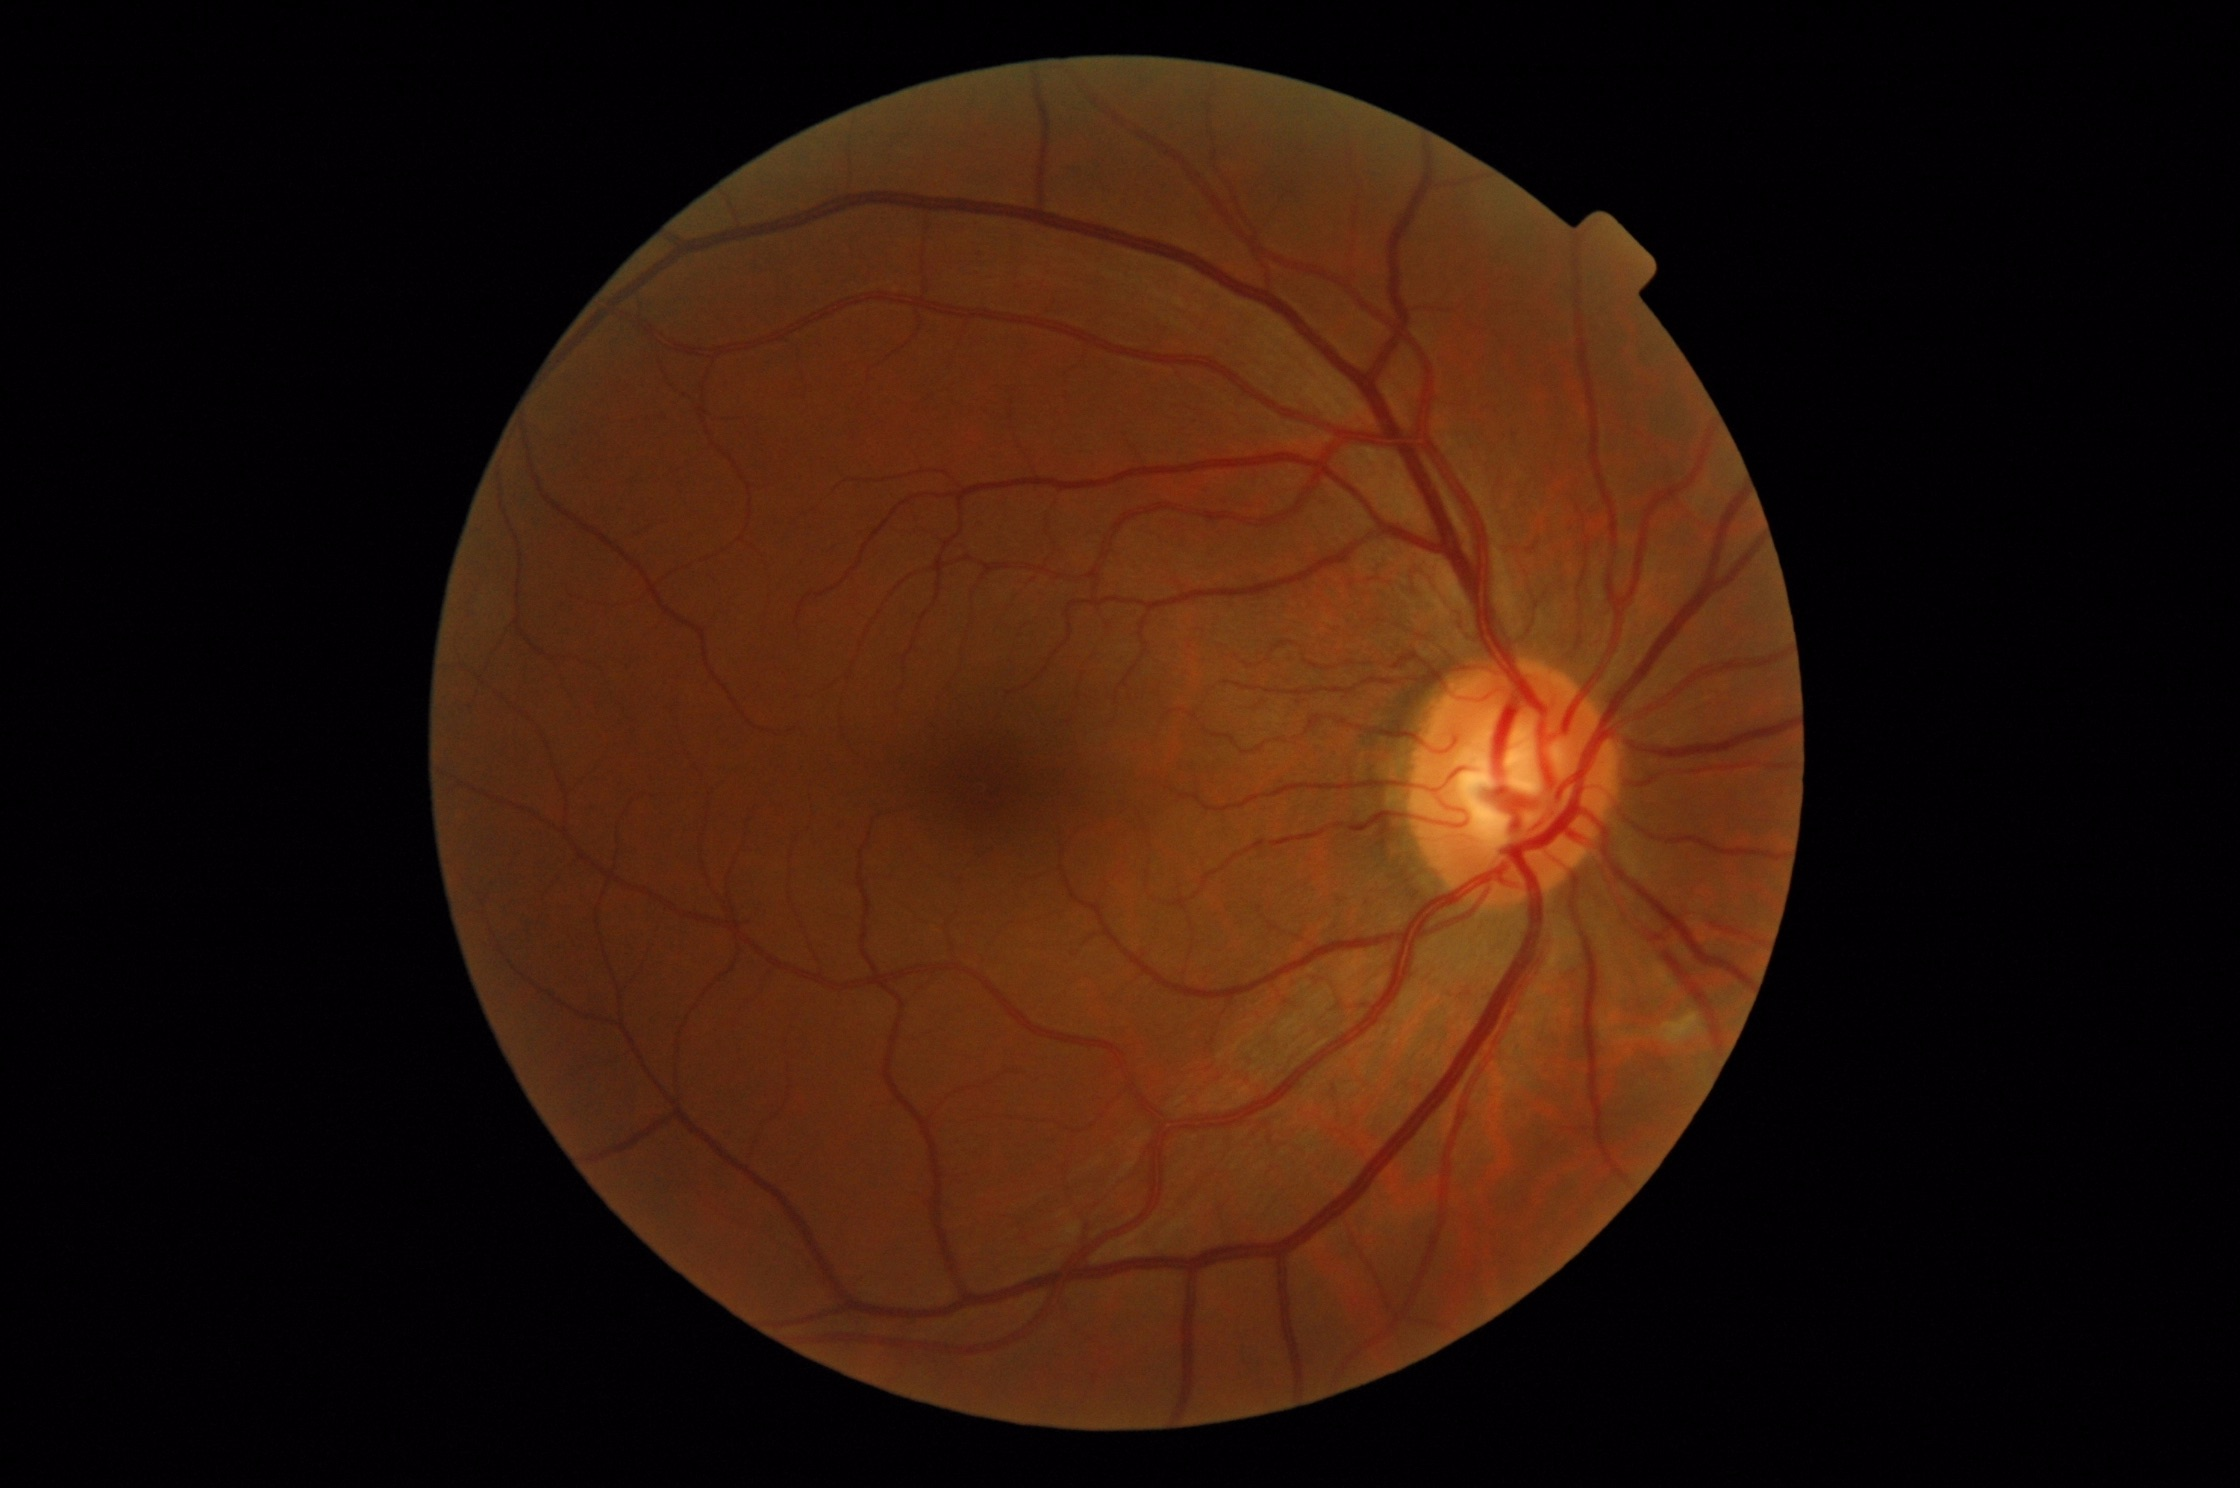
\includegraphics[width=0.8\textwidth]{Figures/NODR}
\caption{withoutDR}
\label{fignoDR}
\end{figure}

\subsection{Neural Networks}
Neural Networks are computational models that are based on the brain architecture to solve different type of problems like image recognition, anomaly detection, signal processing etc.\ \citep{shiffman2012nature}. Basically a neural network is an architecture that has a set of input neurons that are activated by inputs (like pixel RGB values for images) and those inputs are weighted and transformed to the other neurons until the architecture arrives the final output neurons. 

\begin{figure}[t]
\centering
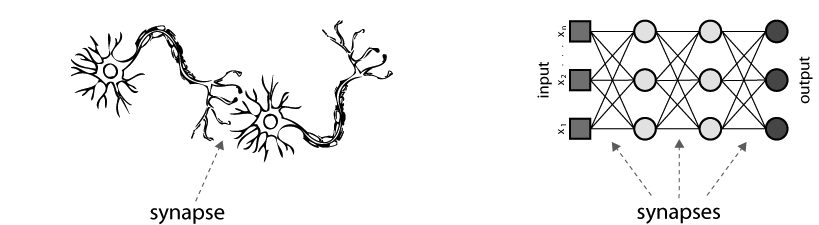
\includegraphics[width=0.8\textwidth]{Figures/nn}
\caption{Neural Network}
\label{fignn}
\end{figure}

Figure~\ref{fignn} shows the similarity between the brain neuron architecture and neural network architecture. 

\subsection{Convolutional Neural Networks}
Convolutional Neural Networks (CNNs) are a type of feed forward neural networks that are based on the animal visual cortex (\url{http://deeplearning.net/tutorial/lenet.html}). CNNs are widely used in different applications of Deep Learning. 
Like regular NNs CNNs also have neurons that have weights and biases that can be learned. The main different between regular NNs and CNNS is that CNNs make the forward function more efficient and creates the neural network architecture with smaller number of parameters learned, which is a lot more efficient (\url{http://cs231n.github.io/convolutional-networks/}).

\begin{figure}[t]
\centering
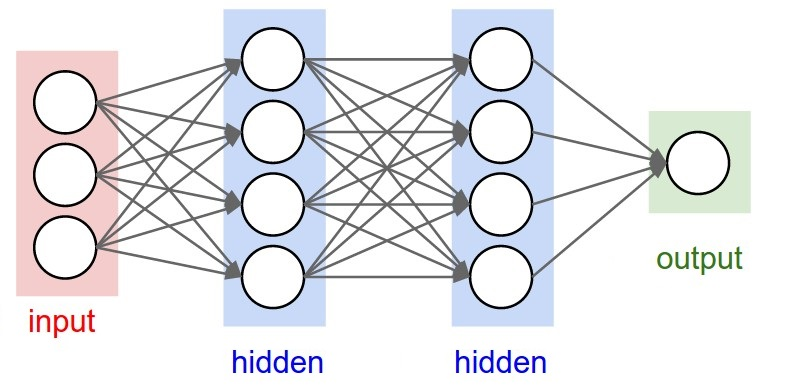
\includegraphics[width=0.8\textwidth]{Figures/regnn}
\caption{Regular Neural Network}
\label{figregnn}
\end{figure}

In Figure~\ref{figregnn} a regular neural network architecture can be seen and Figure~\ref{figconvnet} shows a sample CNN architecture.

\begin{figure}[t]
\centering
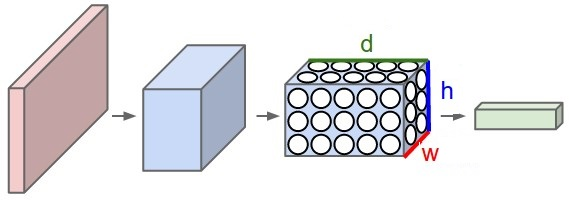
\includegraphics[width=0.8\textwidth]{Figures/convnet}
\caption{Convolutional Neural Network}
\label{figconvnet}
\end{figure}

CNNs are made of different layers that feedforward the activation of the input neurons to the following layers.The layers are as follows:

\begin{enumerate}
    \item Convolutional Layer
    \item Pooling Layer
    \item Fully Connected Layer
\end{enumerate}

To explain the details of the layers of the CNNs we will use a simple CNN architecture for diabetic retinopathy detection problem. Notice that later we will explain the final CNN architecture we use for the classification problem which will have lots of different layers and parameters etc. For now to explain how CNNs are used for detection of signs of diabetic retinopathy we use the following CNN architecture:
\[
\text{INPUT} \Rightarrow \text{CONV} \Rightarrow \text{RELU} \Rightarrow \text{POOL} \Rightarrow \text{FC}.
\]

\begin{description}
    \item[INPUT layer] has the pixel values of the image after preprocessing stage, in our example it is an input image with width 128, height 128 and depth 3 (128x128x3).
    \item[CONV layer] transforms the pixel values of the local regions of the input image by using input neurons' weight and biases. After CONV layer if we use 32 filters, we will have [128x128x32] volume.
    \item[RELU layer] applies an activation function to the output of CONV layer that does not change the volume [128x128x32]
    \item[POOL layer] downsamples the width and height dimensions of the volume resulting in [64x64x32].
    \item[FC layer] classifies the input image to one of the classes (DR and NoDR) resulting in [1x1x2] which has two class scores. Notice that if our problem was to classify input image to 4 classes the output volume would be [1x1x4].
\end{description}


\subsection{TensorFlow}
TensorFlow is a machine learning library opensourced by Google for distributed machine learning and deep learning. In this work for convolutional neural networks we use Google's Tensorflow library (\url{https://www.tensorflow.org}).

\section{Datasets}

In this 

\section{Preprocessing}
Before training the convolutional neural networks the first thing to do is preprocessing the images. Preprocessing is a must stage since the images in the dataset are produced under different circumstances. For instance not all images have the same resolution and not all of the images are produced under the same lightning. To fix these problems we apply some preprocessing techniques for the images. 

\begin{enumerate}
    \item Blur the images. Blurring the images is a technique in Computer Vision problems that is used for enhancing image structures at different scales.
    \item Cropping the images to bounding box having pixel values above a threshold.
    \item Scaling the images to a certain resolution. In our case we scale all of the images to 128x128.
    \item We apply histogram normalization for each of the RGB channels seperately. Histogram normalization changes the pixel intensity values. This results in areas of lower local contrast gaining a higher contrast by effectively spreading out the most frequent intensity values.
\end{enumerate}

TODO: Rotate the images randomly, both test and train data. 
Aplly contrast, sharpness etc to the images and compare the results. 
Add here an image with different preprocessing steps. 

\section{ConvNET Architecture for Diabetic Retinopathy}
In this section we will explain the convolutional neural network used in this work for diabetic retinopathy detection architecture in detail. 

\begin{table}[t]
\centering
\caption{CNN Architecture} \label{tab:cnnarc}
\begin{tabular}{|c|c|c|c|} \hline
\textbf{layer} & \textbf{input volume} & \textbf{no.\ of filters} & \textbf{no.\ of units} \\ \hline
conv & 128$\times$128$\times$3 & 16 & \\ \hline
conv & 128$\times$128$\times$16 & 16 & \\ \hline
pool & 128$\times$128$\times$16 &  & \\ \hline
conv & 64$\times$64$\times$16 & 32 & \\ \hline
conv & 64$\times$64$\times$32 & 32 & \\ \hline
pool & 64$\times$64$\times$32 &  & \\ \hline
conv & 32$\times$32$\times$32 & 64  & \\ \hline
conv & 32$\times$32$\times$64 & 64  & \\ \hline
pool & 32$\times$32$\times$64 &   & \\ \hline
conv & 16$\times$16$\times$64 & 128  & \\ \hline
pool & 16$\times$16$\times$128 &   & \\ \hline
conv & 8$\times$8$\times$128 & 128  & \\ \hline
pool & 8$\times$8$\times$128 &   & \\ \hline
conv & 4$\times$4$\times$128 & 256  & \\ \hline
pool & 4$\times$4$\times$256 &   & \\ \hline
dropout & 2$\times$2$\times$256 & & \\ \hline
fc1 & 2$\times$2$\times$256 & &96 \\ \hline
fc1 & 96$\times$2 & &2 \\ \hline
softmax & & & \\ \hline
\end{tabular}
\end{table}

Table~\ref{tab:cnnarc} shows the details of the convolutional neural network architecture used for this work. Notice that for the number of units after the second fully connected layer, 2 represents number of output classes, in this case DR and noDR. For the degree of the diabetic retinopathy it would be 4. For all of the convolutional layers stride size is 1 and padding is the same, meaning that the dimension (width, height) does not change. Kernel size for conv layers is always 3x3 in this work. Pool layers use maxpooling with 2x2 pooling window and stride is 2, such that after pooling layer width and height is divided by 2. After all convolutinal layers for the activation rectified linear unit (ReLU) is used. (buraya relu image gelecek ve formul) Similarly after the fully connected layer also ReLU is used. 
We trained the net using adam optimizer (a method for stochastic optimization) \citep{kingma2014adam} with  logloss as a loss function. 






\chapter{Evaluation}

In this section we explain the experimental setup, experimental results and discuss the results of the several experiment conducted in detail. 

\section{Evaluation Metrics}
In this section we explain the evaluation metrics used in the experiments. In the experiments we use commonly used evaluation metrics like, sensitivity, specificity, accuracy, roc curve. Table~\ref{tab:configs} shows the possible outcomes of the experiments conducted. True positives are the number of truly detected subjects as abnormal, false negatives are the abnormal subjects but detected as normal by the test. Similarly true negative is number of truly detected subjects as being normal and false positives are subjects that are normal but classified as abnormal by the tests. Notice that depending on the experiments abnormal either means having diabetic retinopathy or having mocelar edema. Definitions of the evaluation metrics are as follows: 

\begin{align*}
    \textit{sensitivity} &= \frac{\textit{TP}}{\textit{TP} + \textit{FN}}
    &
    \textit{specificity} &= \frac{\textit{TN}}{\textit{TN} + \textit{FP}}
\end{align*}

\begin{align*}
    \textit{accuracy} &= \frac{\textit{TP} + \textit{TN}}{\textit{TP} + \textit{FP} + \textit{TN} + \textit{FN}}
\end{align*}

\begin{table}[t]
\centering
\caption{Test subject definitions} 
\label{tab:configs}
\begin{tabular}{|c|c|c|c|} \hline
     & Abnormal & Normal & Total  \\ \hline
     Abnormal& True Positive(TP) & False Positive (FP) & TP + FP \\ \hline
     Normal & False Negative (FN) & True Negative (TN) & TN + FN \\ \hline
     Total & TP + FN &  FP + TN & TP + FN + FP + TN \\ \hline
\end{tabular}
\end{table}

\subsection{Receiver operating characteristic (ROC)}
Another evaluation metric commonly used for diabetic retinopathy research is ROC. ROC is grahical representation of the fraction of TP  vs. FP. TP rate is also known as sensitivity, and FP rate is 1 minus the specificity. 

\subsection{Log Loss}
Logistic loss that is used in neural networks, is the negative log-likelihood of the true labels given a probabilistic classifier’s predictions. For a single sample with true label $\textit{yt} \in \{0,1\}$ and estimated probability $\textit{yp} = P(\textit{yt} = 1)$, the log loss is
\begin{align*}
    -\log P(yt|\textit{yp}) = -(\textit{yt} \log(\textit{yp}) + (1 - \textit{yt}) \log(1 - \textit{yp}))  
\end{align*}

\section{Experimental Configuration}
We run several different experiments with different configurations. Used configurations are as follows:

\begin{itemize}
    \item Nothing: It means images are only scaled to the same size used by the training of the models (128x128 in our experiments). No histogram equalization, enhancement, contrast or rotation is applied to the images. 
    \item Rotate: Both during training and testing images are rotated randomly since in most of the data available, images can belong different eyes (left or right) and their appereance can differ. 
    \item Rotate\_Heq: After random rotation, histogram equalization is applied to all of the images. 
    \item HeqOnly: No rotation is applied to the images, only histogram equalization is used. 
    \item RotateContrast1.5: Medium level of contrast enhancement is applied to the images after random rotation.
    \item RotateContrast1.52: High level of contrast enhancement is applied to the images after random rotation.
    \item AllConf: After random rotation, contrast, sharpen and edge enhance is applied to the image.
\end{itemize}

\section{Experiments with Messidor Dataset}
We run all the experiments in this section by using k-fold cross validation with the settings of k=6. We first shuffle the dataset and split the dataset into 6 folds. Each time we use 80\% of the data as training data and 20\% as test data. We run the following experiments.

\subsection{DR vs NonDR}
Figure \ref{messidoracc} shows accuracy results for Messidor data experiments with average of 6 fold experiments. It can be observed that best configuration is using random rotaion only or AllConf. Almost with 70\% accuracy classifier can truely predict whether eye image contains signs of diabetic retinopathy or not. Table \ref{tab:msdll} shows the logloss values for the experiments. Again the smallest error is obtained by using only rotation.

\begin{figure}[!htbbp]
\centering
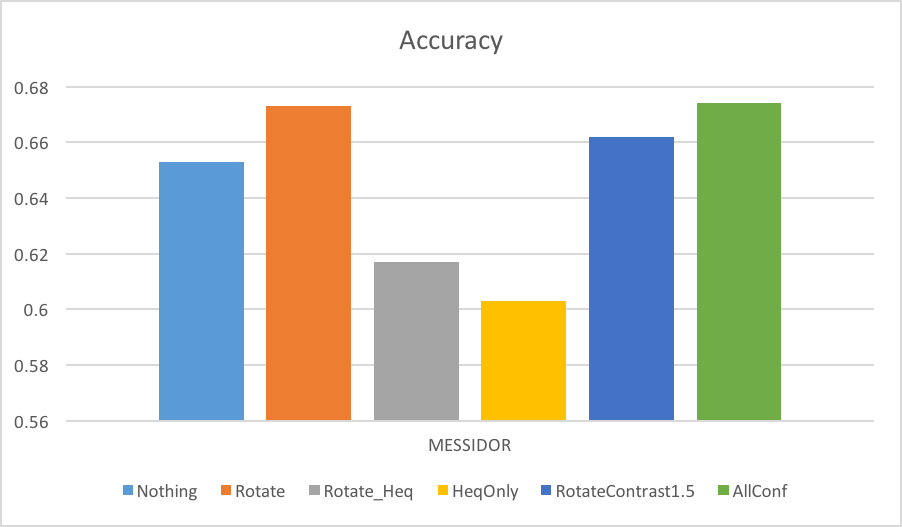
\includegraphics[width=0.8\textwidth]{Figures/messidor.png}
\caption{Accuracy results for Messidor dataset with different preprocessing steps}
\label{messidoracc}
\end{figure}

\begin{table}[t]
\centering
\caption{Messidor Dataset Log Loss values for Experiments} \label{tab:msdll}
\begin{tabular}{|c|c|c|c|c|c|c|} \hline
 & Nothing & Rotate & Rotate\_Heq & HeqOnly & RotateContrast1.5 & AllConf \\ \hline
log loss & 0.68 & 0.654 & 1.024 & 1.002 & 0.762 & 0.686 \\ \hline
\end{tabular}
\end{table}

\subsection{MA vs NonMA}
By looking at the results of the DR NONDR experiments, by using best performed configuration, using only rotation in our case, we run a further experiment for the detection of risk of having macular edema or not. Table \ref{tab:msdma} shows the results.  

\begin{table}[t]
\centering
\caption{Messidor Dataset Experimet Results for MA risk detection} \label{tab:msdma}
\begin{tabular}{|c|c|c|c|c|c|c|} \hline
 Accuracy & Log loss \\ \hline
 0.81 & 0.518\\ \hline
\end{tabular}
\end{table}

\section{Experiments by using other datasets}
In this section we train a convolutional neural network model by using all of the Messidor dataset as training data and test with three different publicly available datasets.
\subsection{Stare Dataset Experiments}
In this part, we show the results of the experiments run with using Messidor dataset as traiing data and Stare dataset as test data. 93 DR and 36 NONDR data. Accuracy results are shown on Figure \ref{stareacc}. ROC graphs for Stare dataset experiments are shown on Figure \ref{stareroc}.\\
Both accuracy results and ROC graphs shows that best configuration is the raw configuration, namely Nothing. Around 70\% of accuracy is obtained and 0.7 area under ROC curve is obtained.   

\begin{figure}[!htbbp]
\centering
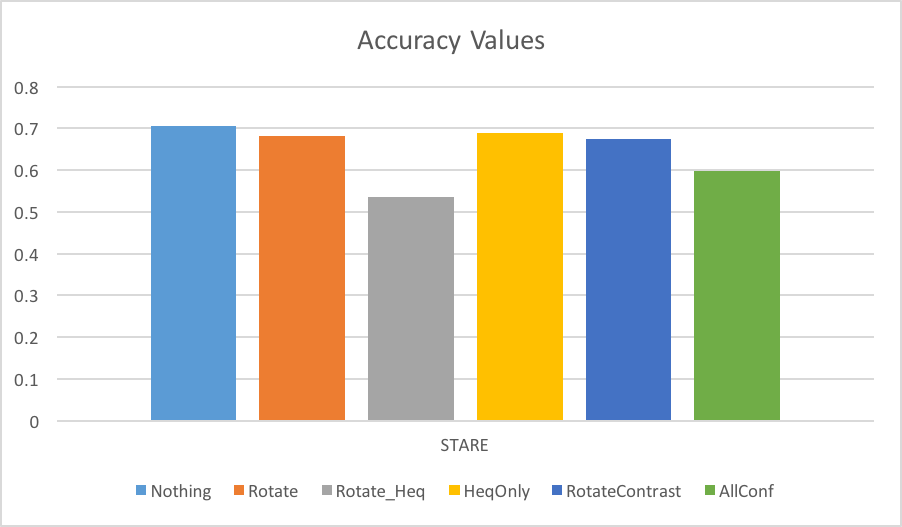
\includegraphics[width=0.8\textwidth]{Figures/stareacc.png}
\caption{Accuracy results for Stare dataset with different preprocessing steps}
\label{stareacc}
\end{figure}

\begin{figure}[!htbbp]
\centering
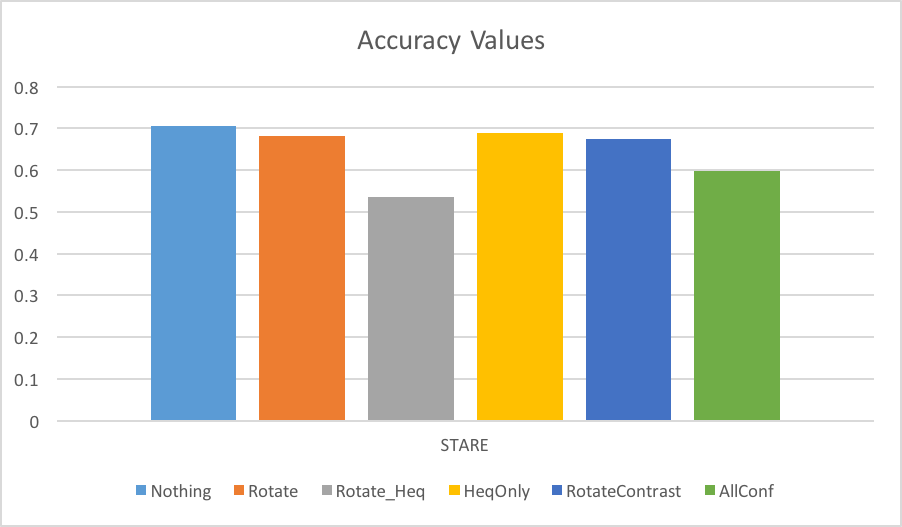
\includegraphics[width=1.0\textwidth]{Figures/stare.png}
\caption{ROC for Stare dataset with different preprocessing steps}
\label{stareroc}
\end{figure}

\subsection{Colour Fundus Images of Healthy Persons \& Patients with Diabetic Retinopathy Dataset(CFI) Experiments}
In this part, we show the results of the experiments run with using Messidor dataset as traiing data and CFI dataset \citep{alipour2012analysis} as test data. 35 DR and 25 NONDR data.\\
Accuracy results are shown on Figure \ref{cfiacc}. ROC graphs for Stare dataset experiments are shown on Figure \ref{cfiroc}.\\
By using random rotation only around 80\% of accuracy results can be obtained and 0.9 area under ROC curve can be obtained with the same configuration. This is one of the best results obtained in our experiments. 

\begin{figure}[!htbbp]
\centering
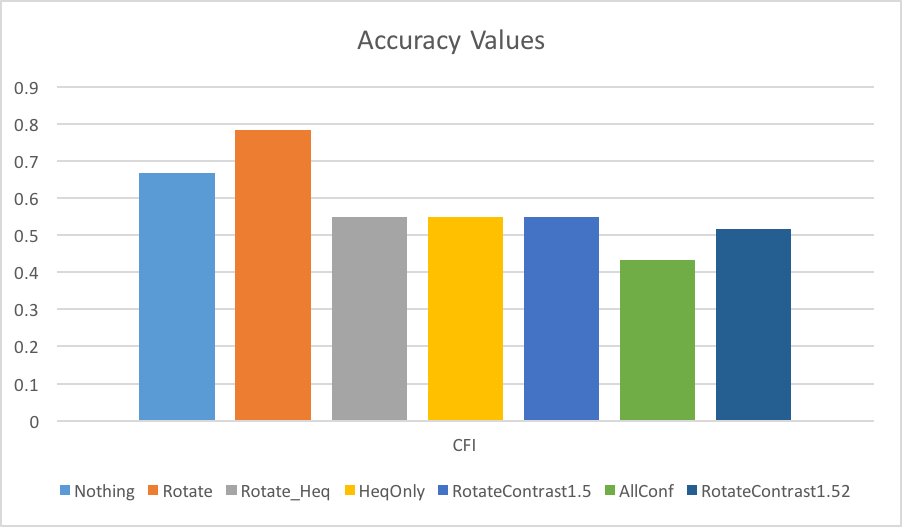
\includegraphics[width=0.8\textwidth]{Figures/cfiacc.png}
\caption{Accuracy results for CFI dataset with different preprocessing steps}
\label{cfiacc}
\end{figure}

\begin{figure}[!htbbp]
\centering
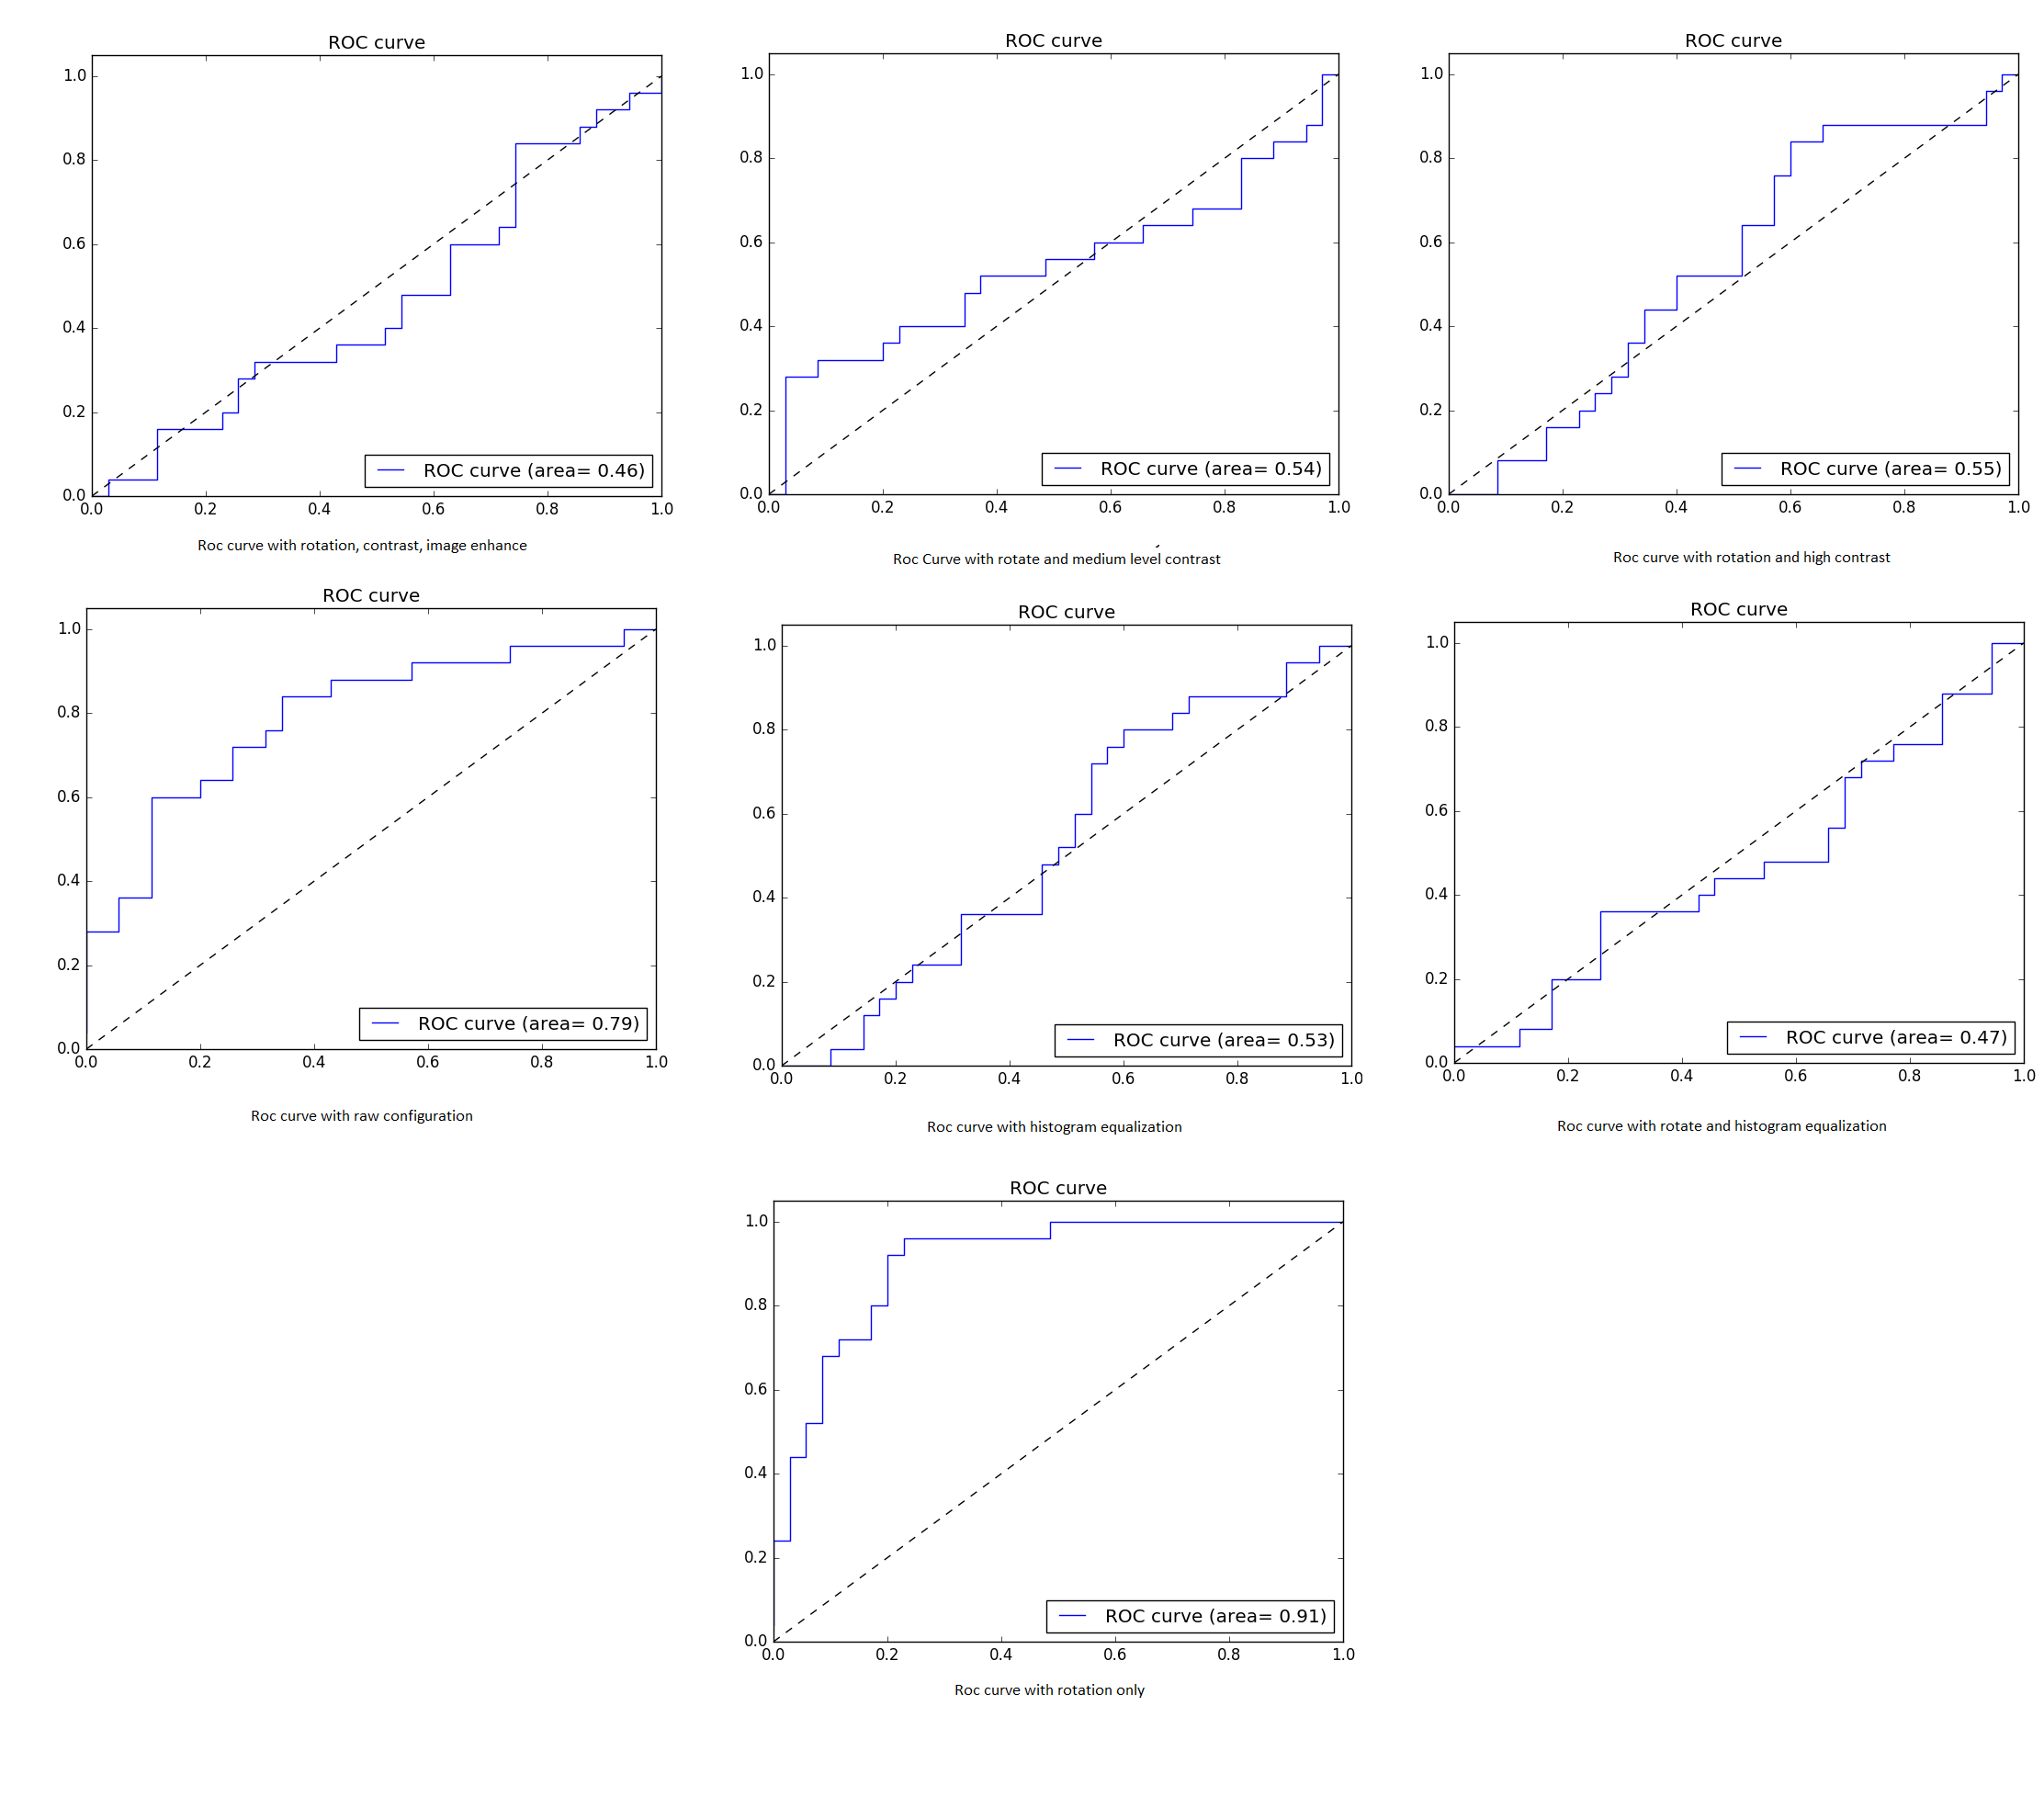
\includegraphics[width=1.0\textwidth]{Figures/cfi.png}
\caption{ROC for CFI dataset with different preprocessing steps}
\label{cfiroc}
\end{figure}


\subsection{High Resolution Fundus Dataset(HRF) Experiments}
In this part, we show the results of the experiments run with using Messidor dataset as traiing data and HRF dataset as test data. 15 DR and 15 NONDR data.\\
Accuracy results are shown on Figure \ref{hrfacc}. ROC graphs for Stare dataset experiments are shown on Figure \ref{hrfroc}.\\
By using raw configuration, applying nothing to the images, around 60\% of accuracy results can be obtained and 0.75 area under ROC curve can be obtained with applying histogram equalization to the images

\begin{figure}[!htbbp]
\centering
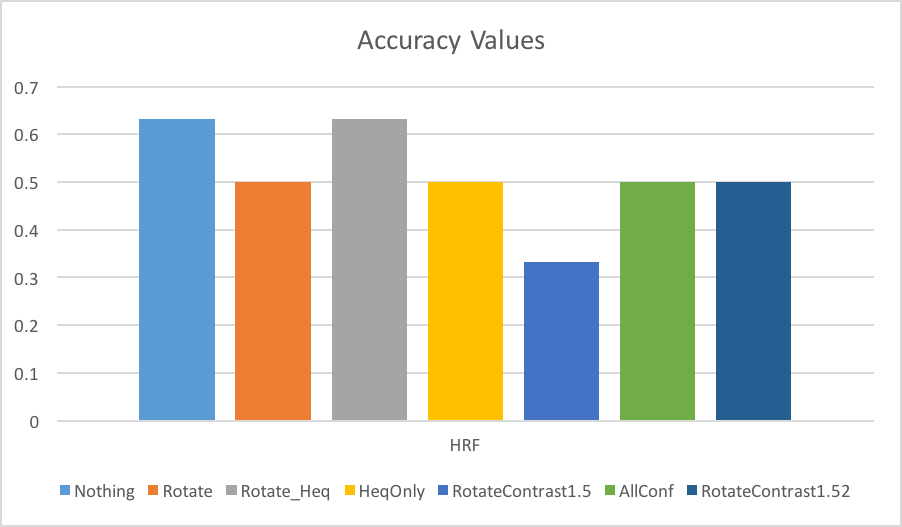
\includegraphics[width=0.8\textwidth]{Figures/hrfacc.png}
\caption{Accuracy results for HRF dataset with different preprocessing steps}
\label{hrfacc}
\end{figure}


\begin{figure}[!htbbp]
\centering
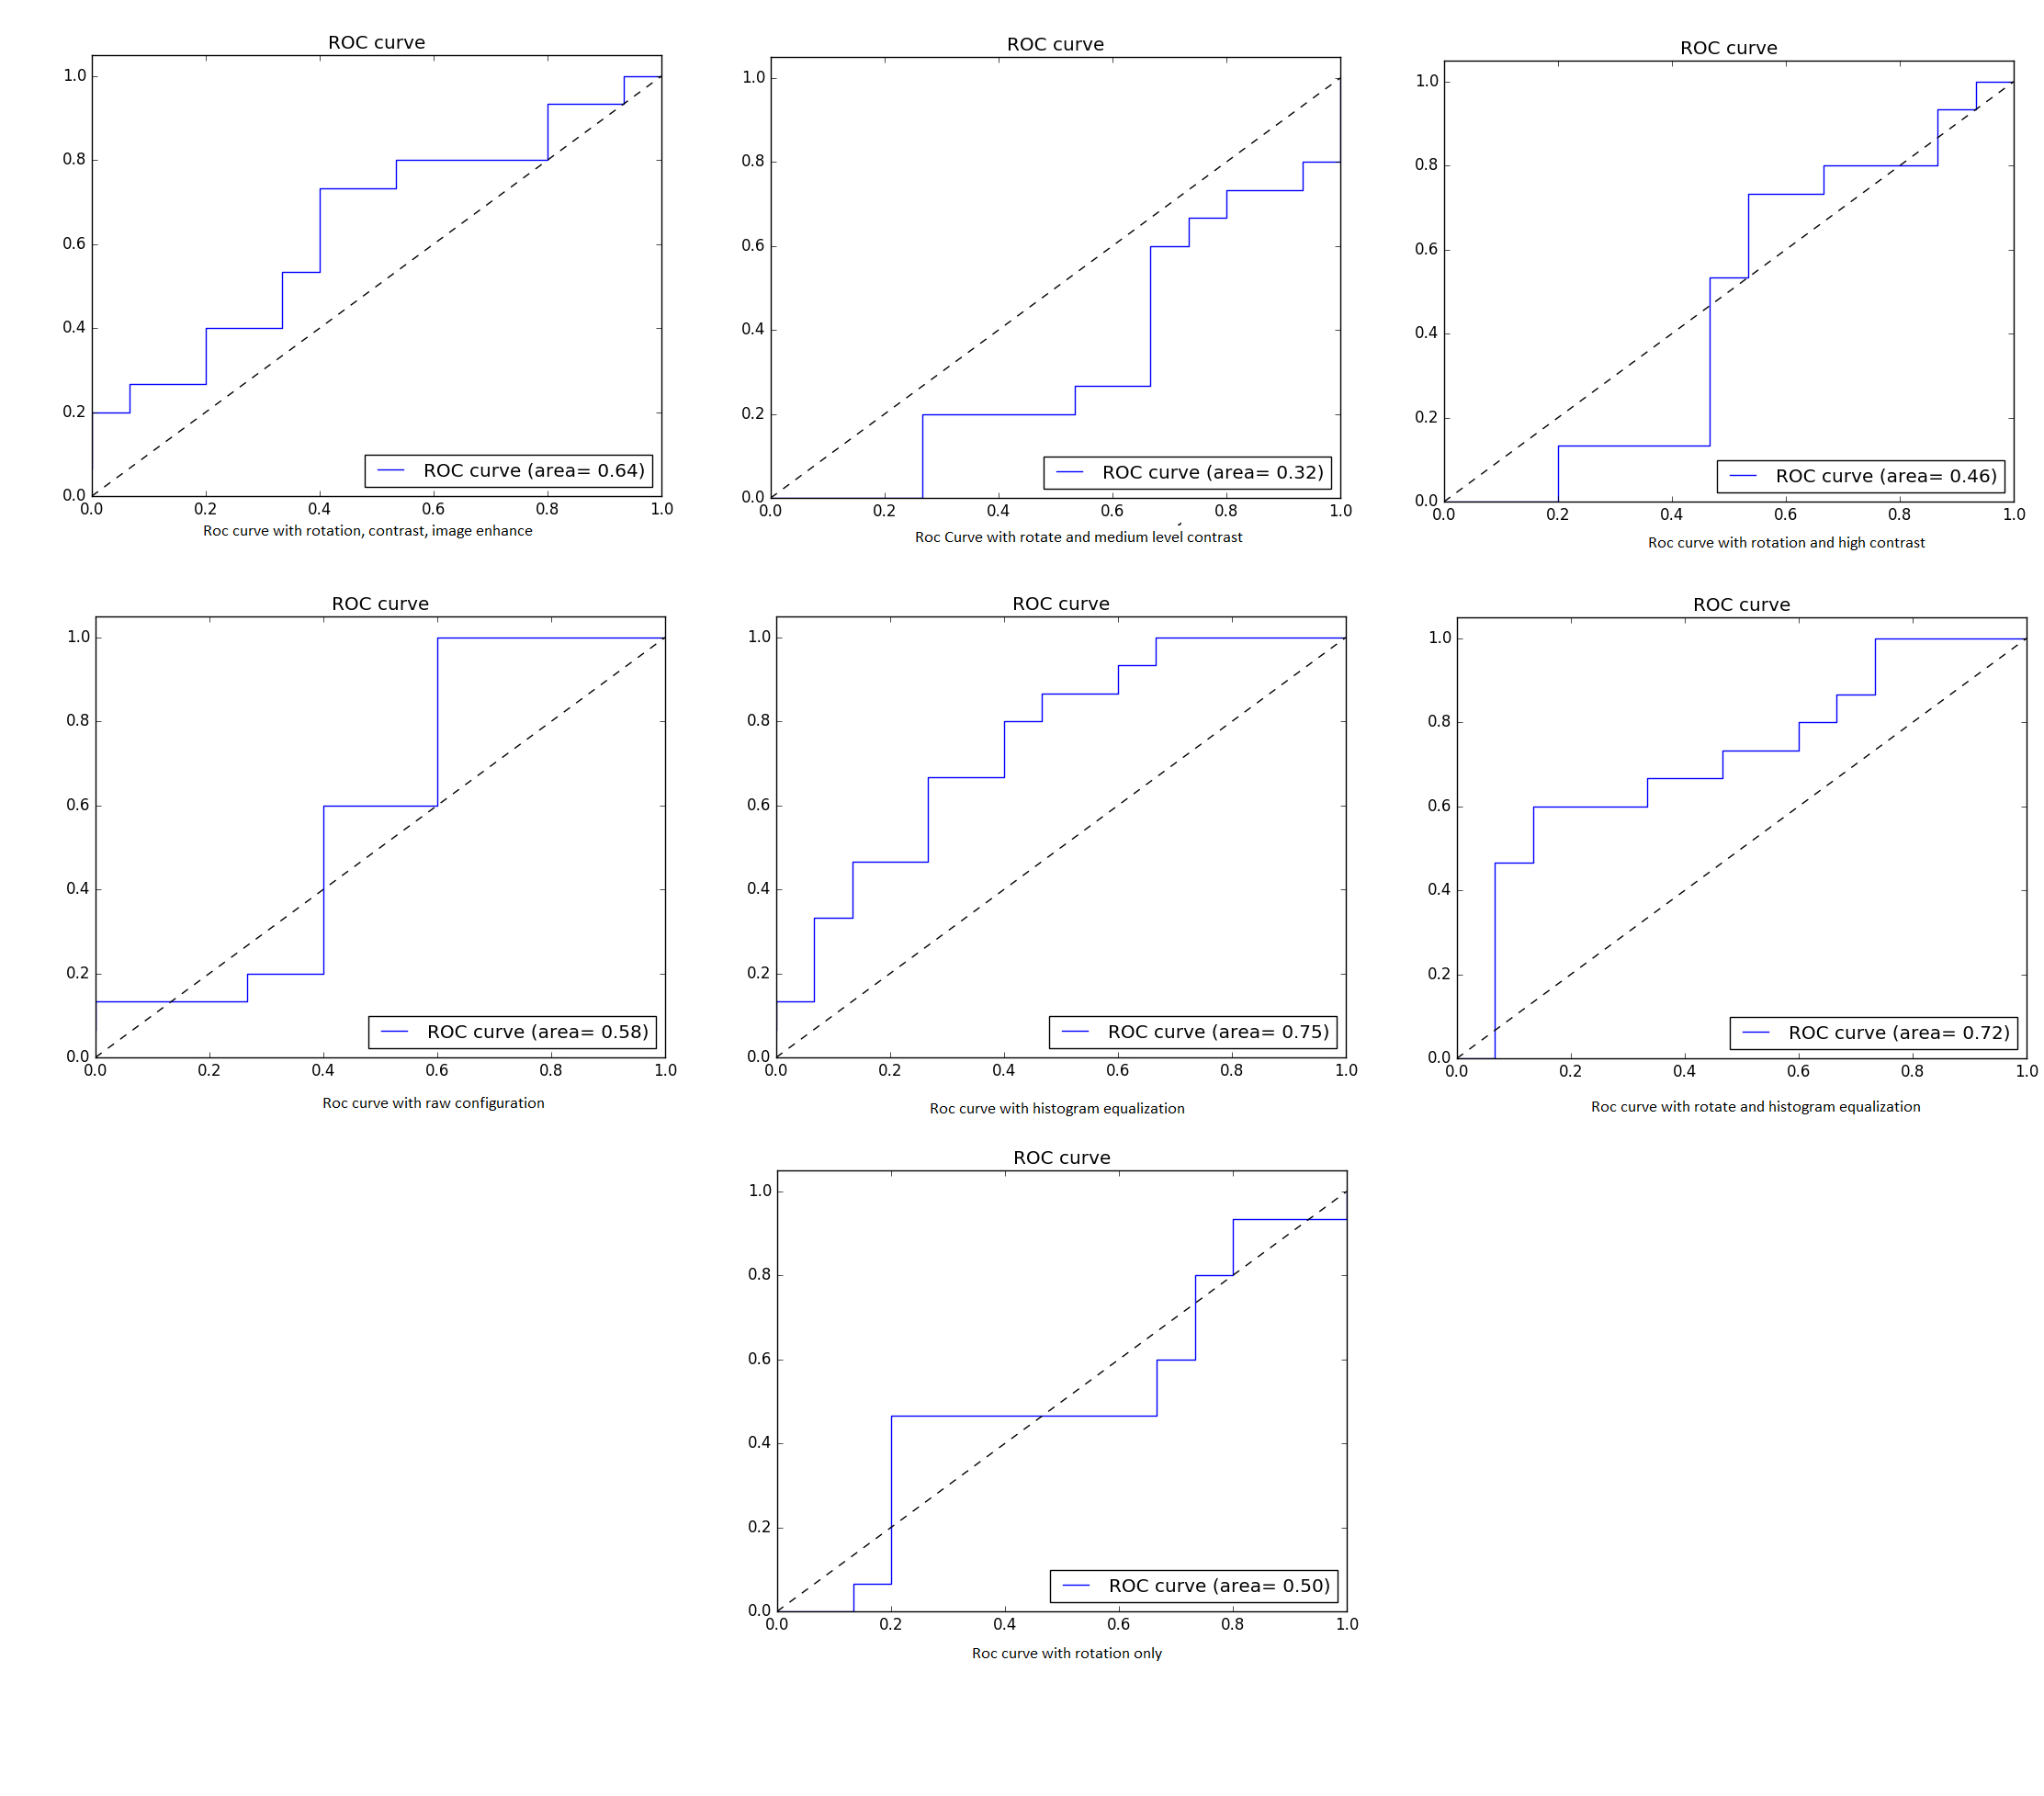
\includegraphics[width=1.0\textwidth]{Figures/hrf.png}
\caption{ROC for HRF dataset with different preprocessing steps}
\label{hrfroc}
\end{figure}


%% \bibliographystyle{apalike}
\bibliographystyle{plainnat} % use this to have URLs listed in References
\cleardoublepage
\bibliography{References/references} % Path to your References.bib file

\end{document}
